% Escala vertical: 0,22 cm por gramo, origen en 996 g.
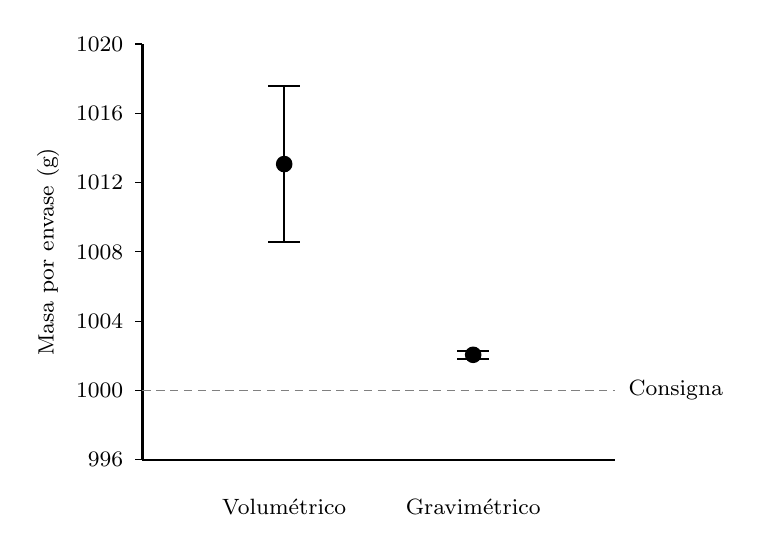
\begin{tikzpicture}[font=\small, nota/.style={font=\footnotesize, align=center}]
\pgfmathsetmacro{\s}{0.22}

% Eje vertical
\draw[thick] (0,0) -- (0,{\s*(1020-996)});
\foreach \g in {996,1000,1004,1008,1012,1016,1020}{
    \draw (0,{\s*(\g-996)}) -- (-0.1,{\s*(\g-996)});
    \node[nota, anchor=east] at (-0.12,{\s*(\g-996)}) {\g};
}
\node[nota, rotate=90] at (-1.2,{\s*12}) {Masa por envase (g)};

% Consigna de 1000 g
\draw[densely dashed, gray] (0,{\s*4}) -- (6,{\s*4});
\node[nota, anchor=west] at (6.05,{\s*4}) {Consigna};

% Volumétrico: media 1013,07 g, desviación 4,5 g
\draw[thick] (1.8,{\s*(1013.07-4.5-996)}) -- (1.8,{\s*(1013.07+4.5-996)});
\draw[thick] (1.6,{\s*(1013.07-4.5-996)}) -- (2.0,{\s*(1013.07-4.5-996)});
\draw[thick] (1.6,{\s*(1013.07+4.5-996)}) -- (2.0,{\s*(1013.07+4.5-996)});
\fill (1.8,{\s*(1013.07-996)}) circle (3pt);
\node[nota] at (1.8,-0.6) {Volumétrico};

% Gravimétrico: media 1002,06 g, desviación 0,24 g
\draw[thick] (4.2,{\s*(1002.06-0.24-996)}) -- (4.2,{\s*(1002.06+0.24-996)});
\draw[thick] (4.0,{\s*(1002.06-0.24-996)}) -- (4.4,{\s*(1002.06-0.24-996)});
\draw[thick] (4.0,{\s*(1002.06+0.24-996)}) -- (4.4,{\s*(1002.06+0.24-996)});
\fill (4.2,{\s*(1002.06-996)}) circle (3pt);
\node[nota] at (4.2,-0.6) {Gravimétrico};

\draw[thick] (0,0) -- (6,0);
\end{tikzpicture}
